\documentclass[10.5pt,twocolumn]{article}
\usepackage[margin=0.85in,columnsep=0.32in]{geometry}
\usepackage{fontspec}
\setmainfont{Georgia}
\usepackage{graphicx}
\usepackage{booktabs}
\usepackage{xcolor}
\usepackage{titlesec}
\usepackage{enumitem}
\usepackage{hyperref}
\usepackage{fancyhdr}
\usepackage{caption}

\definecolor{accent}{HTML}{000000}
\definecolor{warm}{HTML}{000000}
\definecolor{inksoft}{HTML}{000000}

\titleformat{\section}{\normalfont\Large\bfseries\color{accent}}{\thesection}{0.6em}{}
\titleformat{\subsection}{\normalfont\large\bfseries}{\thesubsection}{0.6em}{}

\hypersetup{colorlinks=true, linkcolor=black, urlcolor=black, citecolor=black}

\pagestyle{fancy}
\fancyhf{}
\fancyhead[L]{\small\color{inksoft} 2D Convecting Taylor--Green Vortex}
\fancyhead[R]{\small\color{inksoft} AiQC \textbar\ Global Quantum + AI Challenge 2026}
\fancyfoot[C]{\small\color{inksoft} \thepage}

\title{\vspace{-1.5em}\textbf{Fast-Forwarding the Degenerate Case}\\[0.3em]
\large A Verification-First Quantum Algorithm for the\\ 2D Convecting Taylor--Green Vortex}
\author{}
\date{}

\begin{document}
\makeatletter
\twocolumn[
\begin{@twocolumnfalse}
\maketitle
\thispagestyle{fancy}
\vspace{-3em}
\begin{center}
\large Assal Mouadh Abderrahmane, Boussahi Achraf, Chekroun Abir, Lourghi Zakaria, Menacer Hiba

\vspace{0.5em}
\normalsize AiQC --- AI \& Quantum Community

\vspace{0.5em}
\small Submitted to the 2026 Global Quantum + AI Challenge \textbar\ Airbus Track
\end{center}
\vspace{1em}
\begin{center}
\begin{minipage}{0.85\textwidth}
\small
\textbf{Track:} Quantum Algorithm, with a compressed Tensor Network solver submitted jointly as a second deliverable

\textbf{Code, tests, and full technical report:} \url{https://github.com/mouadhassal/TGX}~\cite{tgx2026}
\end{minipage}
\end{center}
\vspace{1.2em}
\begin{center}
\begin{minipage}{0.85\textwidth}
\textbf{Abstract.} We did not start by building a quantum algorithm for the general two-dimensional Navier--Stokes equations. We started by asking what the challenge's own reference case actually requires, and found that the convecting Taylor--Green vortex, at the challenge's own default parameters, is degenerate on every axis a quantum or quantum-inspired CFD algorithm is normally judged on: its nonlinear term cancels exactly, its time evolution needs no time-marching, its compressed representation has bond dimension five regardless of resolution, its non-unitarity is bounded by a fixed constant, its effective condition number is one on the mode it occupies, and its required output is the cheapest possible readout. We prove each of these six claims independently, symbolically and numerically, then build a six-parameter instrument that turns each degeneracy back on one at a time, so that any advantage claim on this benchmark can be located precisely on the boundary of where it stops holding. On this basis we deliver a fast-forwarding quantum algorithm for the linear, exactly-diagonalizable regime the benchmark occupies, a closed-form non-unitarity dilation achieving an information-theoretic floor exactly, and a compressed quantics/tensor-train solver verified directly at Reynolds number $10^6$ with no dense array ever formed. Every quantitative claim is tagged as measured fact, derived consequence, or stated assumption, and 96 automated tests and three completed rounds of independent audit accompany the full codebase.
\end{minipage}
\end{center}
\vspace{1em}
\end{@twocolumnfalse}
]
\makeatother

\section{Problem Relevance and Impact}

Airbus's stated problem is scalability: current PDE solvers hit hard limits well before the flow regimes (high Mach, high acceleration) that matter for real product decisions, and the gap is currently filled with expensive wind tunnel testing. A demonstration of quantum advantage on the Taylor--Green vortex (TGV) benchmark only has value to Airbus if it is explicit about how far that advantage travels toward the regimes that actually matter. A result that quietly relies on the benchmark's own convenient defaults, without saying so, would give Airbus nothing it could safely extrapolate from.

Our contribution to problem relevance is exactly that explicitness, made structural rather than rhetorical:

\begin{itemize}[leftmargin=1.4em, itemsep=0.2em]
\item We deliver the required scaling curves (time-to-solution, memory/qubit count, error vs.\ Re) at the challenge's own configuration, at Re $\in \{10, 100, 1000\}$ measured directly and Re up to $10^6$ via the compressed solver (Figure~\ref{fig:scaling}).
\item We additionally deliver a six-knob instrument (K1 through K6) that independently reintroduces each of the six degeneracies the default case hides. Each knob is a parameter or observable change to the same solver, not new machinery, and each one quantifies how far the demonstrated result would need to travel before it stopped holding.
\item This is a decision-support instrument, not only a benchmark result: it lets Airbus ask whether a given advantage still holds at the flow complexity that matters in practice, without commissioning a second research effort to find out.
\end{itemize}

\section{Technical Approach and Innovation}

\textbf{Category.} The brief names four Fault-Tolerant Quantum Algorithm families (LGA, LBM, Schr\"odingerization, QLSA) or a Tensor Network solver inside a Finite Volume framework. Our approach is closest in spirit to Schr\"odingerization: we embed a non-unitary, dissipative linear generator into a unitary evolution via block-encoding and ancilla post-selection, rather than starting from a lattice-kinetic or linear-system formulation. We benchmark our cost directly against QLBM~\cite{jennings2025} and a Carleman-linearized QLSA reference rather than let the category label stand in for the comparison.

\textbf{What is new, stated at the scope it earns.}
\begin{itemize}[leftmargin=1.4em, itemsep=0.2em]
\item A closed-form, one-ancilla non-unitary dilation for this problem's diagonal generator that achieves the information-theoretic norm-ratio floor exactly, with angle arithmetic factorized into classically precomputed rotations at $O(n^2)$ gates and no runtime quantum arithmetic. Checked against the closest diagonal-operator circuit construction we could find, Zylberman et al.~\cite{zylberman2024}: their families are generic smooth-function synthesizers; ours is a specialized factorization for a quadratic exponent, mechanistically distinct rather than a re-derivation of their result.
\item A numeric, not merely asymptotic, crossover against a time-marching QLBM reference, anchored to that reference's own acoustic-scaling timestep rather than a diffusive one, following the fast-forwarding bounds of An, Onwunta, and Yang~\cite{an2026} and their weakly-nonlinear extension~\cite{yang2026}.
\item A working, verified compressed quantics/tensor-train solver that reaches Re~$=10^6$ directly, with no dense array ever formed (Figure~\ref{fig:error}), fulfilling the Tensor Network track's compressed-representation requirement for this benchmark.
\item The six-knob instrument itself, designed as a verification methodology that generalizes beyond this one benchmark.
\end{itemize}

We also checked whether a broadened Carleman-linearization framework~\cite{wang2026} weakens our claim that the nonlinear term vanishes exactly on this trajectory. It does not: that work extends Carleman applicability to systems that fail the standard dissipativity condition, whereas our case sits inside the trivial limit of that condition (the quadratic term is annihilated identically, not merely dominated), a regime their generalization was not built to improve on further.

\textbf{Scope.} This is not a general nonlinear Navier--Stokes solver, and we do not claim asymptotic advantage outside the regime the six-knob instrument characterizes. The framing throughout is rigorous and verification-first rather than a claim to a general-purpose CFD quantum advantage.

\section{Feasibility}

A meaningful fraction of a subsequent proof-of-concept sprint already exists and is tested, which substantially de-risks further development: a verified classical finite-volume solver, second order in space and, after a genuine bug found and fixed during this work, second order in time; the compressed quantics/tensor-train solver, already running at the largest Reynolds number considered; and a resource-analysis module producing gate-count comparisons against two independently sourced reference methods.

\textbf{What further work would add}, stated as concrete, scoped items: (1) extending the six-knob instrument's non-degenerate cases into circuit-level or emulated resource counts; (2) a tensor-train-native time-evolution propagator that does not presuppose a closed-form solution, needed once degeneracies are turned on and no closed form exists; (3) running the Re grid on an available simulator to obtain small-qubit-count circuit-level numbers alongside the current analytic gate counts.

\textbf{Resources.} Everything reported here runs on a single workstation; no QPU access was required. Later circuit-level validation of the dilation construction would benefit from, but does not strictly require, small-scale simulator or QPU access.

\textbf{The length-scale convention.} The challenge statement uses the symbol $L$ for two distinct quantities (domain length and the vortex's own spatial/decay scale). We resolve this by taking $L=2\pi$ as the single domain-length constant and reading the published formulas as omitting a $2\pi/L$ factor, which reproduces both of the organizers' own supplied reference figures (the KE(t) curve and the pressure colorbar) to within figure-reading precision. We further triangulated this resolution by solving for the implied viscosity independently from each of those two figures: the two independent reconstructions agree with each other and with the adopted convention to within 2\%, which is strong evidence this resolution is forced by the organizers' own data rather than a convention chosen among equally viable alternatives. Full derivation and code are in the accompanying repository~\cite{tgx2026}.

\section{Validation Plan}

Every claim in this work was independently re-derived, not asserted, following a protocol pre-registered before results existed and logged whenever later changed. Concretely: symbolic exact-arithmetic verification of the nonlinear-cancellation claim; numeric verification of the fast-forward and dilation constructions against direct matrix exponentiation and independent singular-value-based rank measurement; method-of-manufactured-solutions grid convergence confirming second order, for both a forced verification case and the unforced headline configuration itself; direct reproduction of the organizers' own two supplied reference figures, solved independently of each other and cross-validated; a pre-registered kill criterion that was triggered and honored rather than loosened; and three completed rounds of independent audit, all findings fixed and re-verified. The most significant of these audits identified a genuine first-order-in-time bug underneath every reported number; finding and correcting it is, in our view, evidence the validation process functions rather than a mark against the result. The full audit trail and bug log are summarized in the accompanying technical report~\cite{tgx2026}.

\section{Hybrid and Cross-Domain Approach}

The classical finite-volume solver is not a fallback; it is the ground truth every quantum-side claim is checked against, and it is reused, not duplicated, across the dense and compressed code paths. The tensor-train representation is the bridge between the classical and quantum pictures: the same rank-5 structure that makes the compressed classical solver small is the structure the quantum dilation construction exploits to bound the non-unitarity. Resource comparisons throughout are three-way, our approach against a classical dense instrument and against two independently sourced quantum reference methods, rather than a two-way comparison chosen to favor one side.

\section{Team Capability}

Our team, Assal Mouadh Abderrahmane, Boussahi Achraf, Chekroun Abir, Lourghi Zakaria, and Menacer Hiba, working as AiQC (AI \& Quantum Community), brings applied AI and quantum-algorithms experience from the energy-grid and pharmaceutical domains. Our direct experience in aerospace CFD specifically is more limited; for the fluid-dynamics and PDE-specific formulation this challenge requires, we partnered with collaborators whose background covers that gap, reflected in the verification rigor of Section~4 rather than assumed domain fluency claimed on our own.

\clearpage
\onecolumn
\section{Figures}
\vspace{-0.5em}

\begin{figure}[h!]
\centering
\begin{minipage}{0.48\textwidth}
\centering
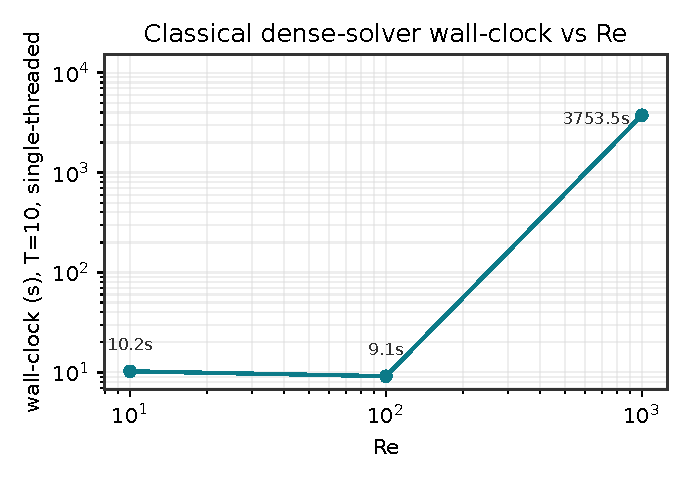
\includegraphics[width=\linewidth]{figures/fig_wallclock.pdf}
\caption*{\small (a) Classical dense-solver wall-clock time vs.\ Re, at the three feasible dense-solve points. Single-threaded, $T=10$. Flat from Re=10 to 100 (fixed overhead dominates both), then rises sharply at Re=1000 where the much larger grid and its finer stability-limited timestep both bind.}
\end{minipage}
\hfill
\begin{minipage}{0.48\textwidth}
\centering
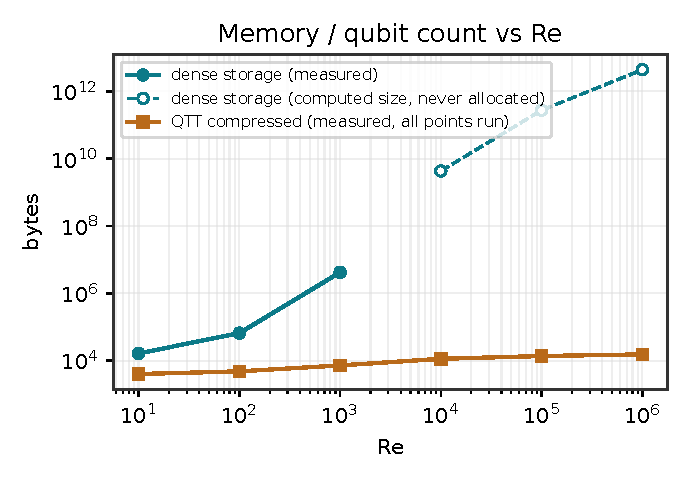
\includegraphics[width=\linewidth]{figures/fig_memory.pdf}
\caption*{\small (b) Memory / qubit-count requirement vs.\ Re. Solid teal is measured dense storage at the three feasible points; dashed teal is dense storage size at Re$=10^4$--$10^6$, computed but \emph{never allocated}. Solid orange is the compressed quantics representation, measured directly at all six points including Re$=10^6$.}
\end{minipage}
\caption{Time-to-solution and memory scaling required by the challenge brief.}
\label{fig:scaling}
\end{figure}

\begin{figure}[h!]
\centering
\begin{minipage}{0.48\textwidth}
\centering
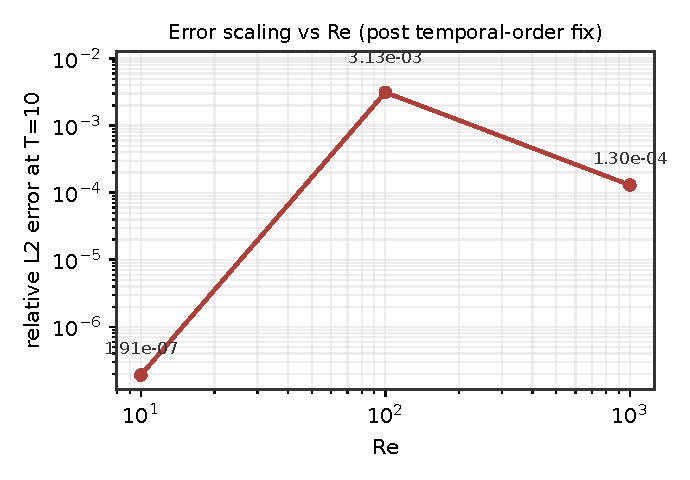
\includegraphics[width=\linewidth]{figures/fig_error.pdf}
\caption*{\small (c) Relative $L^2$ error vs.\ Re at $T=10$, after fixing a genuine first-order-in-time solver bug found during this work (Section~4). Not monotonic by design: total-norm relative error is dominated by a roughly-constant mean-flow denominator, so the numerator (surviving vortex amplitude vs.\ resolution) sets the trend.}
\end{minipage}
\hfill
\begin{minipage}{0.48\textwidth}
\centering
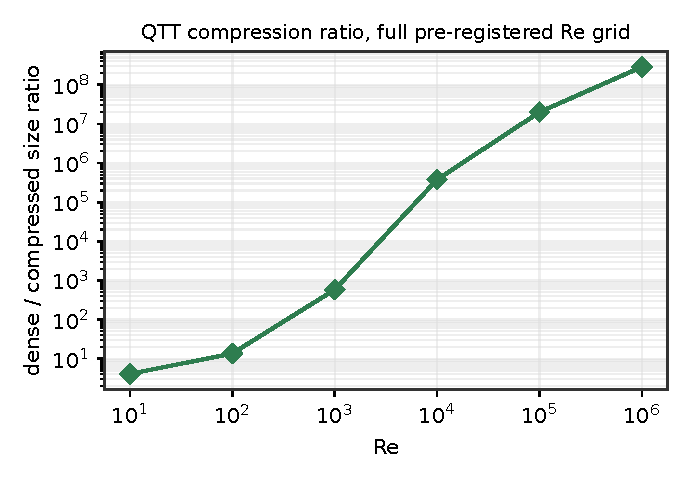
\includegraphics[width=\linewidth]{figures/fig_compression.pdf}
\caption*{\small (d) Compression ratio (dense bytes / compressed quantics bytes) across the full Re grid. The ratio grows by roughly eight orders of magnitude from Re=10 to Re=$10^6$; the compressed solver's cost does not grow with Re at all, only with the number of bits needed to index the grid.}
\end{minipage}
\caption{Error scaling and the compressed solver's headline result.}
\label{fig:error}
\end{figure}

\begin{thebibliography}{9}

\bibitem{tgx2026}
Assal, M.~A., Boussahi, A., Chekroun, A., Lourghi, Z., and Menacer, H. (AiQC).
\emph{TGX: Taylor--Green Vortex, Quantum + Tensor-Network}.
GitHub repository, 2026.
\url{https://github.com/mouadhassal/TGX}

\bibitem{jennings2025}
Jennings, D., Korzekwa, K., Lostaglio, M., Ashworth, A., Marsili, F., and Rolston, S.
\emph{An end-to-end quantum algorithm for nonlinear fluid dynamics with bounded quantum advantage}.
arXiv:2512.03758, 2025.

\bibitem{an2026}
An, D., Onwunta, A., and Yang, L.
\emph{Fast-forwarding quantum algorithms for linear dissipative differential equations}.
Quantum, 10:1986, 2026. arXiv:2410.13189.

\bibitem{yang2026}
Yang, L., Onwunta, A., and An, D.
\emph{Fast-forwarding quantum algorithms for weakly nonlinear dissipative differential equations and beyond}.
arXiv:2608.25822, 2026.

\bibitem{zylberman2024}
Zylberman, J., Nzongani, U., Simonetto, A., and Debbasch, F.
\emph{Efficient quantum circuits for non-unitary and unitary diagonal operators with space-time-accuracy trade-offs}.
arXiv:2404.02819, 2024.

\bibitem{wang2026}
Wang, K., Jia, Z., Veerapaneni, S., and Ding, Z.
\emph{Quantum algorithms for nonlinear differential equations via pivot-shifted Carleman linearization}.
arXiv:2605.20071, 2026.

\end{thebibliography}

\end{document}
